\documentclass[11pt,a4paper]{scrartcl}

\usepackage{amssymb}
\usepackage{amsmath}
\usepackage{yhmath}
\usepackage{tikz}
\usetikzlibrary{angles,quotes,calc,decorations.markings,intersections}
\input{"../../../../9_klase/1. Vienanariai ir daugianariai/manostilius_lt.sty"}

\title{Geometrija I: kampas tarp liestinės ir stygos}
\author{Andrius Berniukevičius}

\begin{document}

\maketitle

\section{Kai apskritimas liečia tiesę}
Ankstesniuose skyriuose kampus siejome apskritimo viduje: taikėme įbrėžtinių kampų ir įbrėžtinių keturkampių savybes. Dabar panagrinėsime, kaip kampų ryšiai pasikeičia, kai prie apskritimo nubrėžiame liestinę.

Olimpiadų uždaviniuose dažnai pasitaiko situacija, kai trikampio ar keturkampio apibrėžtinis apskritimas liečia tiesę. Tokiais atvejais liestinė ir styga sudaro kampą, kurį galima susieti su įbrėžtinu kampu. Ši savybė leidžia perkelti kampo informaciją tarp apskritimo vidaus ir liestinės.

% ==========================================
% BAZINIAI GINKLAI / STRATEGIJOS IR PAVYZDŽIAI
% ==========================================
\section{Pagrindinė teorema}

\begin{definition}
\vocab{Apskritimo liestinė} vadinama tiesė, turinti su apskritimu tik vieną bendrą tašką. Šis taškas vadinamas lietimosi tašku.
\end{definition}

\begin{proposition}[Liestinė ir spindulys]
Jei tiesė $l$ liečia apskritimą taške $A$, o $O$ yra apskritimo centras, tai $OA\perp l$.
\end{proposition}

\begin{proof}
Taikysime prieštaros metodą.

\textbf{1 žingsnis. Pradinis brėžinys.} Turime apskritimą su centru $O$ ir tiesę $l$, kuri liečia apskritimą taške $A$. Pagal liestinės apibrėžimą taškas $A$ yra vienintelis bendras tiesės ir apskritimo taškas. Spindulys $OA$ nubrėžtas į lietimosi tašką.

\begin{center}
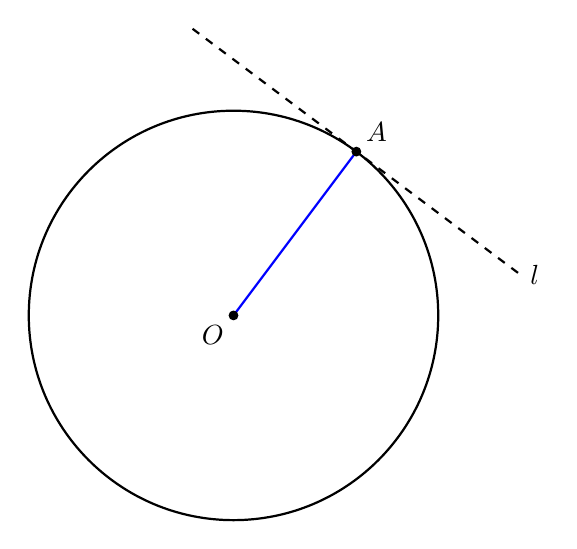
\begin{tikzpicture}[scale=1.3]
    \coordinate (O) at (0,0);
    \coordinate (A) at (1.2,1.6);
    \draw[thick] (O) circle (2);
    \draw[thick, blue] (O) -- (A);
    \draw[thick, dashed] ($(A)+(-1.6,1.2)$) -- ($(A)+(1.6,-1.2)$) node[right] {$l$};
    \filldraw (O) circle (1.2pt) node[below left] {$O$};
    \filldraw (A) circle (1.2pt) node[above right] {$A$};
\end{tikzpicture}
\end{center}

\textbf{2 žingsnis. Prieštaros prielaida.} Tarkime, kad $OA$ nėra statmena tiesei $l$. Iš taško $O$ nubrėžkime atkarpą $OH$ į tiesę $l$ ir tarkime, kad ji yra statmena $l$. Kadangi $OA$ nėra šis statmuo, taškai $H$ ir $A$ nesutampa. Trikampis $OHA$ yra statusis, kurio įžambinė yra $OA$, todėl
\[
OH<OA.
\]

\begin{center}
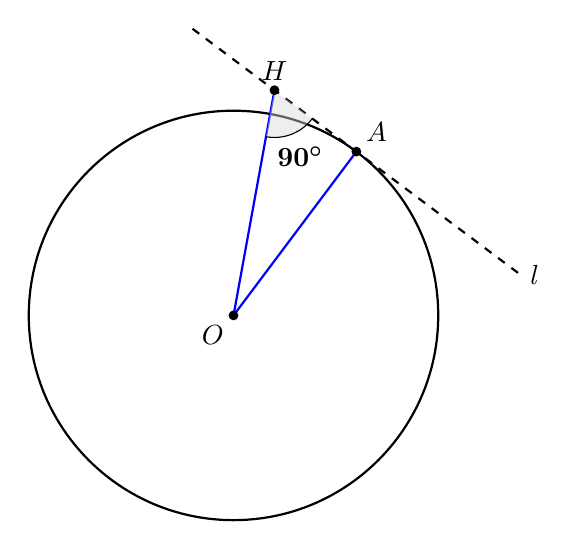
\begin{tikzpicture}[scale=1.3]
    \coordinate (O) at (0,0);
    \coordinate (A) at (1.2,1.6);
    \coordinate (H) at (0.4,2.2);
    \draw[thick] (O) circle (2);
    \draw[thick, blue] (O) -- (A);
    \draw[thick, dashed] ($(A)+(-1.6,1.2)$) -- ($(A)+(1.6,-1.2)$) node[right] {$l$};
    \draw[thick, blue] (O) -- (H);
    \pic [draw=black, fill=black!15, fill opacity=0.45, "$90^\circ$",
        angle radius=6mm, angle eccentricity=1.5,
        pic text options={text=black, text opacity=1, font=\bfseries\boldmath}] {angle = O--H--A};
    \filldraw (O) circle (1.2pt) node[below left] {$O$};
    \filldraw (A) circle (1.2pt) node[above right] {$A$};
    \filldraw (H) circle (1.2pt) node[above] {$H$};
\end{tikzpicture}
\end{center}

\textbf{3 žingsnis. Prieštara.} Brėžinyje matome, kad $OH>OA$: atkarpa $OH$ yra šiek tiek ilgesnė už $OA$. Tačiau trikampis $OHA$ yra statusis, o jo įžambinė turėtų būti $OA$, todėl ji turėtų būti ilgesnė už statinį $OH$. Gavome prieštarą: brėžinyje $OA<OH$, nors stačiajame trikampyje turėtų būti $OA>OH$.
Taigi $OA$ turi būti statmena tiesei $l$.
\end{proof}

\begin{proposition}[Kampas tarp liestinės ir stygos]
Tiesė $l$ liečia apskritimą taške $A$, o $AB$ yra šio apskritimo styga. Jei taškas $C$ priklauso didesniajam lankui $\wideparen{AB}$, tai brėžinyje pažymėtas kampas $\alpha$ tarp $l$ ir $AB$ lygus įbrėžtiniam kampui $\angle ACB$:
\[
\angle ACB = \alpha.
\]
\end{proposition}

\begin{proof}
Įrodymui pasitelksime ką tik įrodytą liestinės ir spindulio statumą bei į skersmenį besiremiančio įbrėžtinio kampo savybę.

\textbf{1 žingsnis.} Apskritimo centras yra \(O\), o tiesė \(l\) liečia apskritimą taške \(A\). Iš taško $A$ nubrėžkime stygą $AB$ ir liestinės bei stygos sudarytą kampą pažymėkime $\alpha$. Ant didesniojo lanko $\wideparen{AB}$ pasirinkime tašką $C$. Įrodysime, kad $\angle ACB=\alpha$.
\begin{center}
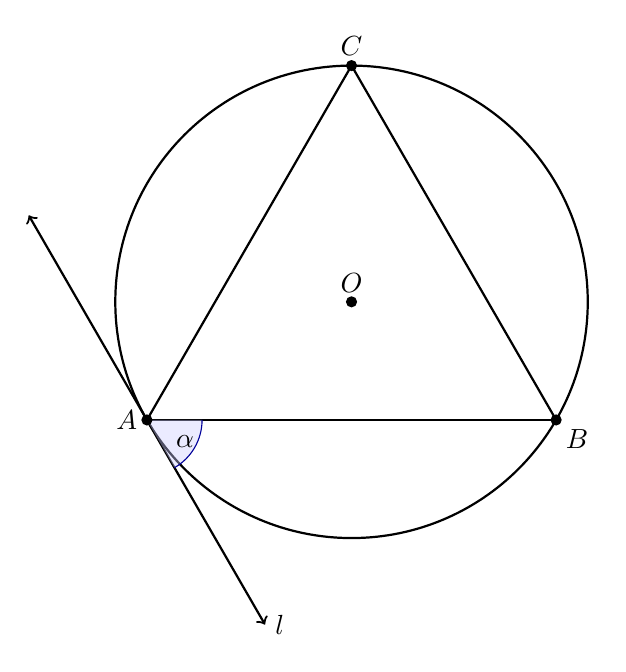
\begin{tikzpicture}[scale=1.5]
    \coordinate (O) at (0,0);
    \draw[thick] (O) circle (2);
    \coordinate (A) at (210:2);
    \coordinate (B) at (330:2);
    \coordinate (C) at (90:2);
    
    % Liestinė
    \coordinate (T1) at ($(A)+(120:2)$);
    \coordinate (T2) at ($(A)+(300:2)$);
    \draw[thick, <->] (T1) -- (T2) node[right] {\(l\)};
    
    \draw[thick] (A) -- (B);
    \draw[thick] (A) -- (C) -- (B);
    
    \pic [draw=blue!60!black, fill=blue!20, fill opacity=0.4, "\(\alpha\)", pic text options={text=black, text opacity=1, opacity=1, font=\bfseries}, angle radius=7mm, angle eccentricity=0.8] {angle = T2--A--B};
    
    \foreach \p/\pos in {O/above, A/left, B/below right, C/above} {
        \filldraw (\p) circle (1.2pt) node[\pos] {\(\p\)};
    }
\end{tikzpicture}
\end{center}

\textbf{2 žingsnis.} Spindulys $OA$ yra statmenas liestinei $l$. Per taškus $O$ ir $A$ nubrėžkime skersmenį $AD$. Kadangi $OA$ yra toje pačioje tiesėje kaip $AD$, tai kampas tarp liestinės ir $AD$ yra statusis. Vadinasi, pagal brėžinyje pažymėtą kampą $\alpha$, $\angle BAD=90^\circ-\alpha$:
\begin{center}
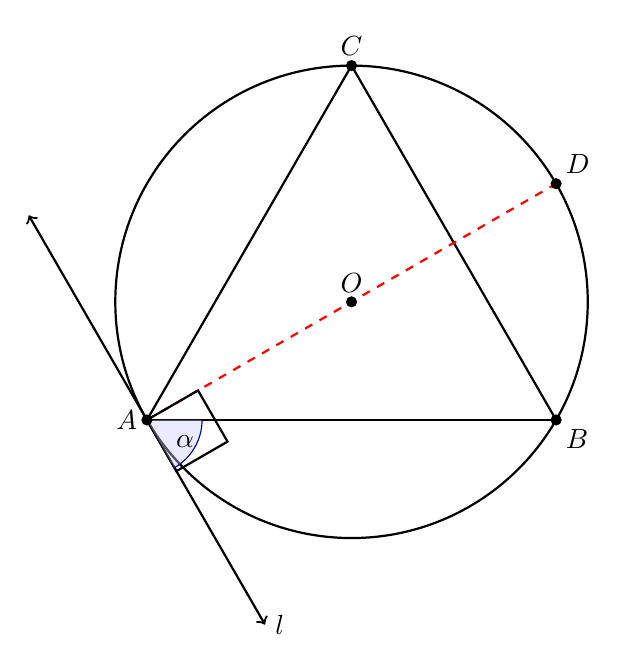
\begin{tikzpicture}[scale=1.5]
    \coordinate (O) at (0,0);
    \draw[thick] (O) circle (2);
    \coordinate (A) at (210:2);
    \coordinate (B) at (330:2);
    \coordinate (C) at (90:2);
    \coordinate (D) at (30:2); % Priešingas A
    
    \coordinate (T1) at ($(A)+(120:2)$);
    \coordinate (T2) at ($(A)+(300:2)$);
    \draw[thick, <->] (T1) -- (T2) node[right] {\(l\)};
    
    \draw[thick] (A) -- (B);
    \draw[thick] (A) -- (C) -- (B);
    \draw[thick, dashed, red] (A) -- (D);
    
    % Statusis kampas tarp liestinės ir skersmens
    \coordinate (dirD) at ($(A)!5mm!(D)$);
    \coordinate (dirT2) at ($(A)!5mm!(T2)$);
    \coordinate (rect) at ($(dirD) + (dirT2) - (A)$);
    \draw[thick, fill=none] (dirD) -- (rect) -- (dirT2) -- (A) -- cycle;
    
    \pic [draw=blue!60!black, fill=blue!20, fill opacity=0.4, "\(\alpha\)", pic text options={text=black, text opacity=1, opacity=1, font=\bfseries}, angle radius=7mm, angle eccentricity=0.8] {angle = T2--A--B};
    
    \foreach \p/\pos in {O/above, A/left, B/below right, C/above, D/above right} {
        \filldraw (\p) circle (1.2pt) node[\pos] {\(\p\)};
    }
\end{tikzpicture}
\end{center}

\textbf{3 žingsnis.} Sujunkime taškus $D$ ir $B$. Kadangi $AD$ yra skersmuo, į jį besiremiantis kampas $\angle ABD$ yra statusis. Trikampyje $\triangle ABD$ kampų suma lygi $180^\circ$, todėl
\[
\angle ADB=180^\circ-90^\circ-(90^\circ-\alpha)=\alpha.
\]
\begin{center}
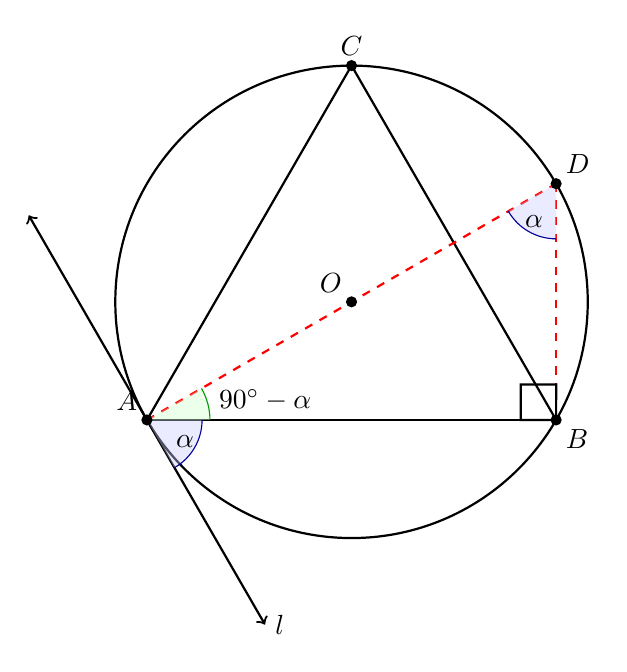
\begin{tikzpicture}[scale=1.5]
    \coordinate (O) at (0,0);
    \draw[thick] (O) circle (2);
    \coordinate (A) at (210:2); \coordinate (B) at (330:2); \coordinate (C) at (90:2); \coordinate (D) at (30:2);
    
    \coordinate (T1) at ($(A)+(120:2)$); \coordinate (T2) at ($(A)+(300:2)$);
    \draw[thick, <->] (T1) -- (T2) node[right] {\(l\)};
    
    \draw[thick] (A) -- (B); \draw[thick] (A) -- (C) -- (B);
    \draw[thick, dashed, red] (A) -- (D); \draw[thick, dashed, red] (D) -- (B);
    
    \coordinate (dirA_B) at ($(B)!3mm!(A)$); \coordinate (dirD_B) at ($(B)!3mm!(D)$); \coordinate (rectB) at ($(dirA_B) + (dirD_B) - (B)$);
    \draw[thick, fill=none] (dirA_B) -- (rectB) -- (dirD_B) -- (B) -- cycle;
    
    \pic [draw=blue!60!black, fill=blue!20, fill opacity=0.4, "\(\alpha\)", pic text options={text=black, text opacity=1, opacity=1, font=\bfseries}, angle radius=7mm, angle eccentricity=0.8] {angle = T2--A--B};
    \pic [draw=green!60!black, fill=green!20, fill opacity=0.4, "\(90^\circ-\alpha\)", pic text options={text=black, text opacity=1, opacity=1, font=\bfseries, xshift=-2mm,yshift = -2mm}, angle radius=8mm, angle eccentricity=2.2] {angle = B--A--D};
    \pic [draw=blue!60!black, fill=blue!20, fill opacity=0.4, "\(\alpha\)", pic text options={text=black, text opacity=1, opacity=1, font=\bfseries}, angle radius=7mm, angle eccentricity=0.8] {angle = A--D--B};
    
    \foreach \p/\pos in {O/above left, A/above left, B/below right, C/above, D/above right} {
        \filldraw (\p) circle (1.2pt) node[\pos] {\(\p\)};
    }
\end{tikzpicture}
\end{center}

\textbf{4 žingsnis.} Kampai $\angle ADB$ ir $\angle ACB$ remiasi į tą patį lanką $\wideparen{AB}$, todėl jie lygūs. Kadangi $\angle ADB=\alpha$, gauname $\angle ACB=\alpha$.
\begin{center}
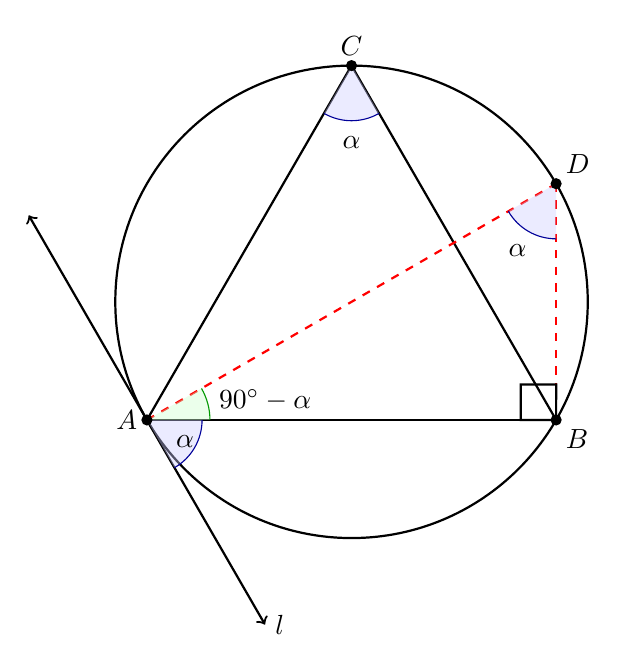
\begin{tikzpicture}[scale=1.5]
    \coordinate (O) at (0,0);
    \draw[thick] (O) circle (2);
    \coordinate (A) at (210:2); \coordinate (B) at (330:2); \coordinate (C) at (90:2); \coordinate (D) at (30:2);
    
    \coordinate (T1) at ($(A)+(120:2)$); \coordinate (T2) at ($(A)+(300:2)$);
    \draw[thick, <->] (T1) -- (T2) node[right] {\(l\)};
    
    \draw[thick] (A) -- (B); \draw[thick] (A) -- (C) -- (B);
    \draw[thick, dashed, red] (A) -- (D); \draw[thick, dashed, red] (D) -- (B);

    \coordinate (dirA_B) at ($(B)!3mm!(A)$);
    \coordinate (dirD_B) at ($(B)!3mm!(D)$);
    \coordinate (rectB) at ($(dirA_B) + (dirD_B) - (B)$);
    \draw[thick, fill=none] (dirA_B) -- (rectB) -- (dirD_B) -- (B) -- cycle;
    
    \pic [draw=blue!60!black, fill=blue!20, fill opacity=0.4, "\(\alpha\)", pic text options={text=black, text opacity=1, opacity=1, font=\bfseries}, angle radius=7mm, angle eccentricity=0.8] {angle = T2--A--B};
    \pic [draw=green!60!black, fill=green!20, fill opacity=0.4, "\(90^\circ-\alpha\)", pic text options={text=black, text opacity=1, opacity=1, font=\bfseries, xshift=-2mm, yshift=-2mm}, angle radius=8mm, angle eccentricity=2.2] {angle = B--A--D};
    \pic [draw=blue!60!black, fill=blue!20, fill opacity=0.4, "\(\alpha\)", pic text options={text=black, text opacity=1, opacity=1, font=\bfseries}, angle radius=7mm, angle eccentricity=1.4] {angle = A--D--B};
    \pic [draw=blue!60!black, fill=blue!20, fill opacity=0.4, "\(\alpha\)", pic text options={text=black, text opacity=1, opacity=1, font=\bfseries}, angle radius=7mm, angle eccentricity=1.4] {angle = A--C--B};
    
    \foreach \p/\pos in {A/left, B/below right, C/above, D/above right} {
        \filldraw (\p) circle (1.2pt) node[\pos] {\(\p\)};
    }
\end{tikzpicture}
\end{center}
Įrodyta. Taigi kampas tarp liestinės ir stygos lygus įbrėžtiniam kampui, kuris remiasi į tą pačią stygą. \hfill \(\square\)
\end{proof}

% ==========================================
% BENDROJI LIESTINĖ
% ==========================================
\section{Pavyzdys: dviejų apskritimų konfigūracija}
Liestinės ir stygos kampo savybę galima taikyti ir tada, kai uždavinyje nagrinėjami du besiliečiantys apskritimai. Per jų lietimosi tašką nubrėžta bendroji liestinė padeda susieti abiejų apskritimų kampus.

\begin{example}[Besiliečiantys apskritimai ir lygiagrečios stygos]
Du apskritimai liečiasi išorėje taške \(T\). Per tašką \(T\) nubrėžta kirstinė, kuri kerta pirmąjį apskritimą taške \(A\), o antrąjį – taške \(B\). Iš taškų \(A\) ir \(B\) nubrėžtos liestinės šiems apskritimams (atitinkamai tiesės \(l_1\) ir \(l_2\)). Įrodykite, kad šios liestinės yra lygiagrečios (\(l_1 \parallel l_2\)).
\end{example}

\begin{proof}
\textbf{Sprendimas.} Per lietimosi tašką $T$ nubrėšime bendrąją liestinę $m$. Tada nuosekliai pritaikysime liestinės ir stygos kampo savybę abiem apskritimams.

\textbf{1 žingsnis.} Pradiniame brėžinyje turime du apskritimus, jų lietimosi tašką \(T\), kirstinę \(ATB\) ir dvi liestines. Lygiagretumo kol kas nežymime, nes jį reikia įrodyti. Per tašką \(T\) nubrėžkime pagalbinę tiesę \(m\), kuri liečia abu apskritimus (bendroji liestinė).
\begin{center}
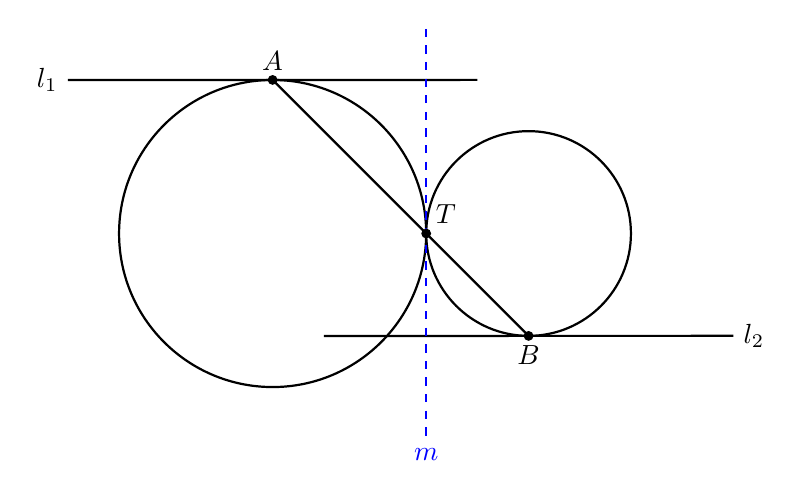
\begin{tikzpicture}[scale=1.3]
    \coordinate (O1) at (-1.5, 0);
    \coordinate (O2) at (1, 0);
    \draw[thick] (O1) circle (1.5);
    \draw[thick] (O2) circle (1);
    
    \coordinate (T) at (0,0);
    % Kirstinė pasukta taip, kad kampas su liestinėmis būtų 45 laipsniai
    \coordinate (A) at (-1.5, 1.5);
    \coordinate (B) at (1, -1);
    
    \draw[thick] (A) -- (B);
    
    % Liestinė per A
    \coordinate (dirA) at ($(A)!1!90:(O1)$);
    \draw[thick] ($(A)!2cm!(dirA)$) -- ($(A)!-2cm!(dirA)$) node[left] {\(l_1\)};
    
    % Liestinė per B
    \coordinate (dirB) at ($(B)!1!90:(O2)$);
    \draw[thick] ($(B)!2cm!(dirB)$) -- ($(B)!-2cm!(dirB)$) node[right] {\(l_2\)};
    
    % Bendra liestinė m
    \draw[thick, dashed, blue] (0, 2) -- (0, -2) node[below] {\(m\)};
    
    \foreach \p/\pos in {T/above right, A/above, B/below} {
        \filldraw (\p) circle (1.2pt) node[\pos] {\(\p\)};
    }
\end{tikzpicture}
\end{center}

\textbf{2 žingsnis.} Nagrinėkime kairįjį apskritimą. Atkarpa $AT$ yra jo styga, o $l_1$ – liestinė taške $A$. Pažymėkime kampą tarp $l_1$ ir $AT$ raide $\alpha$. Pagal liestinės ir stygos teoremą šis kampas lygus įbrėžtiniam kampui, besiremiančiam į stygą $AT$. Ta pati savybė leidžia lyginti kampus, kuriuos styga $AT$ sudaro su liestinėmis jos galuose. Todėl kampas tarp $AT$ ir bendrosios liestinės $m$ taške $T$ taip pat lygus $\alpha$:
\begin{equation*}
\angle (l_1, AT) = \angle (m, AT) = \alpha 
\end{equation*}
\begin{center}
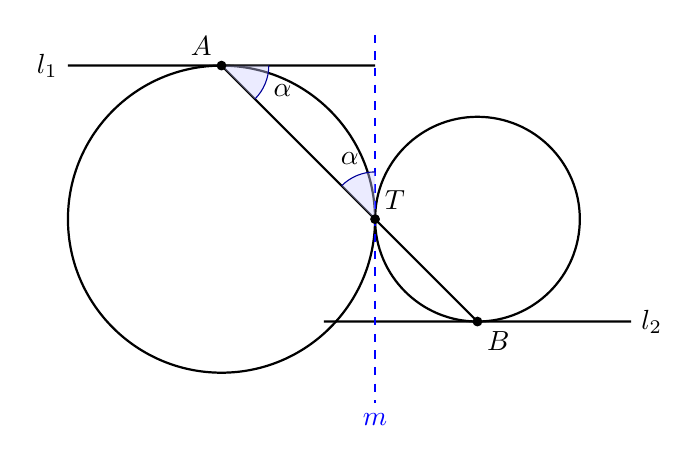
\begin{tikzpicture}[scale=1.3]
    \coordinate (O1) at (-1.5, 0);
    \coordinate (O2) at (1, 0);
    \draw[thick] (O1) circle (1.5);
    \draw[thick] (O2) circle (1);
    \coordinate (T) at (0,0);
    \coordinate (A) at (-1.5, 1.5);
    \coordinate (B) at (1, -1);
    
    \draw[thick] (A) -- (B);
    \coordinate (dirA) at ($(A)!1!90:(O1)$);
    \coordinate (l1_top) at ($(A)!1.5cm!(dirA)$);
    \coordinate (l1_bot) at ($(A)!-1.5cm!(dirA)$);
    \draw[thick] (l1_top) -- (l1_bot) node[left] {\(l_1\)};
    
    \coordinate (dirB) at ($(B)!1!90:(O2)$);
    \draw[thick] ($(B)!1.5cm!(dirB)$) -- ($(B)!-1.5cm!(dirB)$) node[right] {\(l_2\)};
    
    \coordinate (m_top) at (0, 1.8);
    \draw[thick, dashed, blue] (m_top) -- (0, -1.8) node[below] {\(m\)};
    
    % Kampai
    \pic [draw=blue!60!black, fill=blue!20, fill opacity=0.4, "\(\alpha\)", pic text options={text=black, text opacity=1, opacity=1, font=\bfseries}, angle radius=6mm, angle eccentricity=1.4] {angle = T--A--l1_top};
    \pic [draw=blue!60!black, fill=blue!20, fill opacity=0.4, "\(\alpha\)", pic text options={text=black, text opacity=1, opacity=1, font=\bfseries}, angle radius=6mm, angle eccentricity=1.4] {angle = m_top--T--A};
    
    \foreach \p/\pos in {T/above right, A/above left, B/below right} {
        \filldraw (\p) circle (1.2pt) node[\pos] {\(\p\)};
    }
\end{tikzpicture}
\end{center}

\textbf{3 žingsnis.} Tiesės $AB$ ir $m$ susikerta taške $T$, todėl kampas tarp $m$ ir $AT$ lygus jam priešingajam kryžminiam kampui tarp $m$ ir $TB$. Taigi ir dešiniajame apskritime kampas tarp bendrosios liestinės $m$ ir stygos $TB$ yra $\alpha$.
\begin{center}
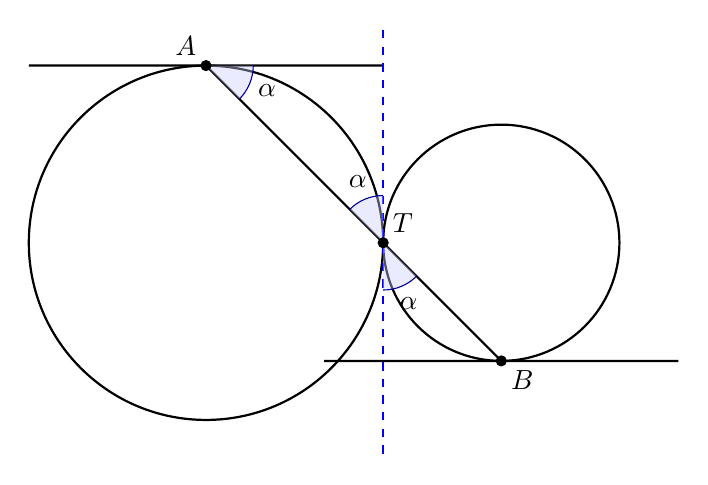
\begin{tikzpicture}[scale=1.5]
    \coordinate (O1) at (-1.5, 0); \coordinate (O2) at (1, 0);
    \draw[thick] (O1) circle (1.5); \draw[thick] (O2) circle (1);
    \coordinate (T) at (0,0); \coordinate (A) at (-1.5, 1.5); \coordinate (B) at (1, -1);
    
    \draw[thick] (A) -- (B);
    \coordinate (dirA) at ($(A)!1!90:(O1)$); \coordinate (l1_top) at ($(A)!1.5cm!(dirA)$); \coordinate (l1_bot) at ($(A)!-1.5cm!(dirA)$);
    \draw[thick] (l1_top) -- (l1_bot);
    
    \coordinate (dirB) at ($(B)!1!90:(O2)$); \coordinate (l2_top) at ($(B)!1.5cm!(dirB)$); \coordinate (l2_bot) at ($(B)!-1.5cm!(dirB)$);
    \draw[thick] (l2_top) -- (l2_bot);
    
    \coordinate (m_top) at (0, 1.8); \coordinate (m_bot) at (0, -1.8);
    \draw[thick, dashed, blue] (m_top) -- (m_bot);
    
    \pic [draw=blue!60!black, fill=blue!20, fill opacity=0.4, "\(\alpha\)", pic text options={text=black, text opacity=1, opacity=1, font=\bfseries}, angle radius=6mm, angle eccentricity=1.4] {angle = T--A--l1_top};
    \pic [draw=blue!60!black, fill=blue!20, fill opacity=0.4, "\(\alpha\)", pic text options={text=black, text opacity=1, opacity=1, font=\bfseries}, angle radius=6mm, angle eccentricity=1.4] {angle = m_top--T--A};
    \pic [draw=blue!60!black, fill=blue!20, fill opacity=0.4, "\(\alpha\)", pic text options={text=black, text opacity=1, opacity=1, font=\bfseries}, angle radius=6mm, angle eccentricity=1.4] {angle = m_bot--T--B};
    
    \foreach \p/\pos in {T/above right, A/above left, B/below right} {
        \filldraw (\p) circle (1.2pt) node[\pos] {\(\p\)};
    }
\end{tikzpicture}
\end{center}

\textbf{4 žingsnis.} Dešiniajame apskritime $m$ yra liestinė taške $T$, o $TB$ – styga. Pagal liestinės ir stygos teoremą kampas tarp $m$ ir $TB$ lygus kampui tarp $TB$ ir liestinės $l_2$ taške $B$. Vadinasi, pastarasis kampas taip pat lygus $\alpha$.
\begin{center}
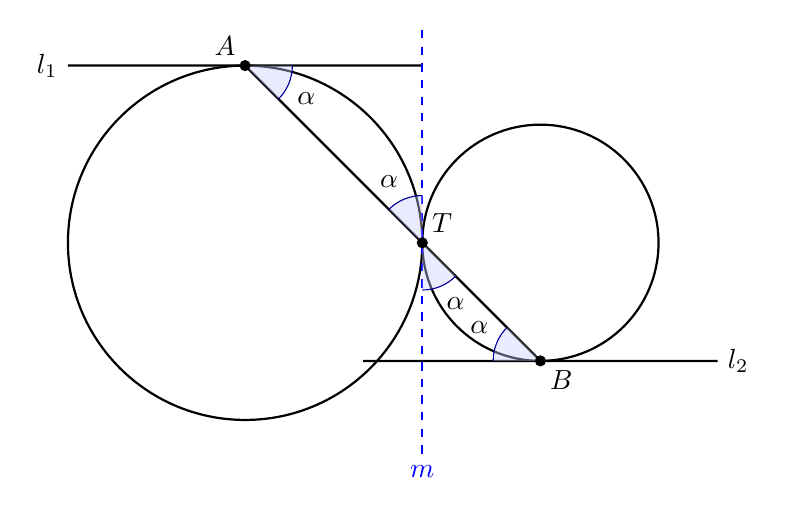
\begin{tikzpicture}[scale=1.5]
    \coordinate (O1) at (-1.5, 0); \coordinate (O2) at (1, 0);
    \draw[thick] (O1) circle (1.5); \draw[thick] (O2) circle (1);
    \coordinate (T) at (0,0); \coordinate (A) at (-1.5, 1.5); \coordinate (B) at (1, -1);
    
    \draw[thick] (A) -- (B);
    \coordinate (dirA) at ($(A)!1!90:(O1)$); \coordinate (l1_top) at ($(A)!1.5cm!(dirA)$); \coordinate (l1_bot) at ($(A)!-1.5cm!(dirA)$);
    \draw[thick] (l1_top) -- (l1_bot) node[left] {\(l_1\)};
    
    \coordinate (dirB) at ($(B)!1!90:(O2)$); \coordinate (l2_top) at ($(B)!1.5cm!(dirB)$); \coordinate (l2_bot) at ($(B)!-1.5cm!(dirB)$);
    \draw[thick] (l2_top) -- (l2_bot) node[right] {\(l_2\)};
    
    \coordinate (m_top) at (0, 1.8); \coordinate (m_bot) at (0, -1.8);
    \draw[thick, dashed, blue] (m_top) -- (m_bot) node[below] {\(m\)};
    
    \pic [draw=blue!60!black, fill=blue!20, fill opacity=0.4, "\(\alpha\)", pic text options={text=black, text opacity=1, opacity=1, font=\bfseries,yshift  =-1mm}, angle radius=6mm, angle eccentricity=1.4] {angle = T--A--l1_top};
    \pic [draw=blue!60!black, fill=blue!20, fill opacity=0.4, "\(\alpha\)", pic text options={text=black, text opacity=1, opacity=1, font=\bfseries,xshift = -1mm}, angle radius=6mm, angle eccentricity=1.4] {angle = m_top--T--A};
    \pic [draw=blue!60!black, fill=blue!20, fill opacity=0.4, "\(\alpha\)", pic text options={text=black, text opacity=1, opacity=1, font=\bfseries, xshift = 1mm}, angle radius=6mm, angle eccentricity=1.4] {angle = m_bot--T--B};
    \pic [draw=blue!60!black, fill=blue!20, fill opacity=0.4, "\(\alpha\)", pic text options={text=black, text opacity=1, opacity=1, font=\bfseries,yshift = 1mm}, angle radius=6mm, angle eccentricity=1.4] {angle = T--B--l2_top};
    
    \foreach \p/\pos in {T/above right, A/above left, B/below right} {
        \filldraw (\p) circle (1.2pt) node[\pos] {\(\p\)};
    }
\end{tikzpicture}
\end{center}

Kirstinė $AB$ kerta tieses $l_1$ ir $l_2$, o gauti vidaus priešiniai kampai yra lygūs. Todėl pagal lygiagrečių tiesių požymį $l_1\parallel l_2$.

Įrodyta. \hfill \(\square\)
\end{proof}

\vspace{0.5cm}

% ==========================================
% UŽDAVINIAI
% ==========================================
\newpage
\section{Uždaviniai savarankiškam sprendimui (30 iššūkių)}

\setlist[enumerate]{itemsep=0.55em, topsep=0.6em, parsep=0pt}

\begin{enumerate}
    \renewcommand{\labelenumi}{\textbf{\theenumi.}}

    \item Apskritimas liečia tiesę taške $A$, o $AB$ yra jo styga. Mažesnysis kampas tarp liestinės ir stygos $AB$ lygus $40^\circ$. Taškas $C$ priklauso didesniajam lankui $\wideparen{AB}$. Raskite kampo $ACB$ dydį.
    \item Tiesė $l$ liečia apskritimą taške $A$, o $AB$ yra styga. Mažesniojo lanko $\wideparen{AB}$ laipsninis matas yra $110^\circ$. Raskite mažesnįjį kampą tarp tiesės $l$ ir stygos $AB$.
    \item Trikampis $ABC$ įbrėžtas į apskritimą, o tiesė $l$ liečia apskritimą taške $A$. Žinoma, kad $\angle ABC=\angle ACB=55^\circ$. Įrodykite, kad $l\parallel BC$.
    \item Iš išorinio taško $P$ nubrėžta apskritimo liestinė $PT$ (čia $T$ – lietimosi taškas) ir kirstinė, kuri apskritimą kerta taškuose $A$ ir $B$ tokia tvarka: $P,A,B$. Įrodykite, kad $\angle PTA=\angle TBA$.
    \item Du apskritimai liečiasi viduje taške $K$. Tiesė per $K$ kerta mažesnįjį apskritimą dar taške $A$, o didesnįjį – dar taške $B$. Įrodykite, kad apskritimų liestinės taškuose $A$ ir $B$ yra lygiagrečios.
    \item Tiesė $l$ liečia trikampio $ABC$ apibrėžtinį apskritimą taške $A$ ir yra lygiagreti kraštinei $BC$. Įrodykite, kad $AB=AC$.
    \item Tiesė $l$ liečia apskritimą taške $T$, o $CD$ yra šio apskritimo styga, lygiagreti $l$. Įrodykite, kad trikampis $TCD$ yra lygiašonis.
    \item Iš taško $P$, esančio už apskritimo, nubrėžtos liestinės $PA$ ir $PB$, kur $A$ ir $B$ – lietimosi taškai. Taškas $C$ priklauso mažesniajam lankui $\wideparen{AB}$. Įrodykite, kad $\angle ACB=90^\circ+\frac{1}{2}\angle APB$.
    \item Taškai $A,B,C,D$ priklauso vienam apskritimui, o stygos $AB$ ir $CD$ kertasi taške $E$. Apskritimo liestinė taške $A$ yra lygiagreti tiesei $CD$. Įrodykite, kad $\angle AEC=\angle ACB$.
    \item Apskritimai $\omega_1$ ir $\omega_2$ liečiasi išoriškai taške $T$. Tiesė per $T$ kerta $\omega_1$ dar taške $A$, o $\omega_2$ – dar taške $B$. Kita tiesė per $T$ kerta $\omega_1$ dar taške $C$, o $\omega_2$ – dar taške $D$. Įrodykite, kad $AC\parallel BD$.
\end{enumerate}

\begin{enumerate}
    \setcounter{enumi}{10}
    \item Tiesė $l$ liečia apskritimą taške $A$, $AB$ yra styga, o $AC$ – skersmuo. Kampas tarp tiesių $AB$ ir $AC$ lygus $30^\circ$. Raskite mažesnįjį kampą tarp $l$ ir $AB$.
    \item Trikampio $ABC$ įbrėžto apskritimo centras yra $I$. Tiesė $AI$ kerta trikampio apibrėžtinį apskritimą antrą kartą taške $W$. Įrodykite, kad apibrėžtinio apskritimo liestinė taške $W$ yra lygiagreti $BC$.
    \item Apskritimai $\omega_1$ ir $\omega_2$ kertasi taškuose $P$ ir $Q$. Apskritimo $\omega_1$ liestinė taške $P$ kerta $\omega_2$ dar taške $A$, o apskritimo $\omega_2$ liestinė taške $P$ kerta $\omega_1$ dar taške $B$. Įrodykite, kad $\angle AQP=\angle BQP$.
    \item Įbrėžtinio keturkampio $ABCD$ įstrižainės $AB$ ir $CD$ kertasi taške $K$. Iš $K$ nuleisti statmenys į tieses $AC$ ir $AD$; jų pagrindai atitinkamai yra $E$ ir $F$. Įrodykite, kad taškai $A,E,K,F$ priklauso vienam apskritimui.
    \item Trikampio $ABC$ apibrėžtinio apskritimo liestinė taške $C$ kerta tiesę $AB$ taške $D$. Žinoma, kad $CD=CB$. Įrodykite, kad $\angle ACD=\angle ABC$.
    \item Taškai $A,B,C,D$ priklauso vienam apskritimui, o $l$ yra šio apskritimo liestinė taške $A$. Žinoma, kad kampas tarp $l$ ir $AB$ lygus $\angle CAD$. Įrodykite, kad stygos $AB$ ir $CD$ yra lygios.
    \item Smailiajame trikampyje $ABC$ atkarpa $BD$ yra statmena $AC$, o $CE$ – statmena $AB$. Įrodykite, kad trikampio apibrėžtinio apskritimo liestinė taške $A$ yra lygiagreti $DE$.
    \item Apskritimas $\omega_1$ liečia apskritimą $\omega_2$ iš vidaus taške $T$. Styga $AB$ priklauso $\omega_2$ ir liečia $\omega_1$ taške $P$. Įrodykite, kad $TP$ yra kampo $ATB$ pusiaukampinė.
    \item Taškai $A,B,C,D$ priklauso vienam apskritimui. Liestinės taškuose $A$ ir $B$ kertasi taške $P$, o liestinės taškuose $C$ ir $D$ – taške $Q$. Apskritimo centras priklauso tiesei $PQ$. Įrodykite, kad $AB\parallel CD$.
    \item Iš taško $P$, esančio už apskritimo $\omega$, nubrėžtos dvi liestinės $PA$ ir $PB$, o kirstinė per $P$ kerta $\omega$ taškuose $C$ ir $D$ ($C$ yra arčiau $P$). Įrodykite, kad $PA^2=PC\cdot PD$.
\end{enumerate}

\begin{enumerate}
    \setcounter{enumi}{20}
    \item Trikampis $ABC$ įbrėžtas į apskritimą. Apskritimo liestinės taškuose $B$ ir $C$ kertasi taške $P$. Įrodykite, kad mažesnysis kampas tarp šių liestinių lygus $\lvert180^\circ-2\angle BAC\rvert$.
    \item Du apskritimai $\omega_1$ ir $\omega_2$ kertasi taškuose $A$ ir $B$. Tiesė per $A$ kerta $\omega_1$ dar taške $C$, o $\omega_2$ – dar taške $D$. Apskritimų liestinės taškuose $C$ ir $D$ kertasi taške $P$. Įrodykite, kad keturkampis $CBDP$ yra įbrėžtinis.
    \item Į apskritimą įbrėžtas lygiakraštis trikampis $ABC$. Taškas $P$ priklauso mažesniajam lankui $\wideparen{BC}$. Liestinė apskritimui taške $P$ kerta tieses $AB$ ir $AC$ atitinkamai taškuose $M$ ir $N$. Įrodykite, kad trikampiai $AMN$ ir $ABC$ yra panašūs.
    \item Tiesė $l$ liečia trikampio $ABC$ apibrėžtinį apskritimą taške $A$. Taškas $D$ priklauso atkarpai $BC$. Apskritimas per taškus $A,B,D$ liečia tiesę $AC$ taške $A$. Įrodykite, kad $l\parallel AD$.
    \item Apskritimai $\omega_1$ ir $\omega_2$ liečiasi išoriškai taške $T$. Tiesė per $T$ kerta $\omega_1$ dar taške $A$, o $\omega_2$ – dar taške $B$. Kita tiesė per $T$ kerta $\omega_1$ dar taške $C$, o $\omega_2$ – dar taške $D$. Įrodykite, kad $\angle ATC+\angle BTD=180^\circ$.
    \item Trikampis $ABC$ statusis, $\angle ACB=90^\circ$. Apskritimas, kurio skersmuo yra $BC$, kerta įžambinę $AB$ dar taške $D$. Šio apskritimo liestinė taške $D$ kerta tiesę $AC$ taške $M$. Įrodykite, kad $M$ yra atkarpos $AC$ vidurio taškas.
    \item Keturkampis $ABCD$ yra įbrėžtinis, o jo įstrižainės $AC$ ir $BD$ kertasi taške $P$. Apibrėžtinio apskritimo liestinės taškuose $A$ ir $B$ kertasi taške $K$. Taškai $K,P,C,D$ priklauso vienam apskritimui. Raskite mažesnįjį kampą tarp liestinių.
    \item Taškai $P,A,B$ priklauso vienam apskritimui, o $PA$ ir $PB$ yra stygos. Iš taško $P$ nuleistų statmenų į apskritimo liestines taškuose $A$ ir $B$ pagrindai yra atitinkamai $M$ ir $N$. Įrodykite, kad $PM=PN$.
    \item Trikampis $ABC$ įbrėžtas į apskritimą. Apskritimo liestinės taškuose $B$ ir $C$ kertasi taške $T$, o tiesė $AT$ kerta kraštinę $BC$ taške $M$. Tiesė $AT$ antrą kartą kerta apskritimą taške $N$. Įrodykite, kad $N$ yra lanko $BC$, kuriame nėra taško $A$, vidurio taškas.
    \item \textbf{Archimedo dvyniai.} Apskritimai $\omega$ ir $\omega'$ liečia tą pačią tiesę $l$ taške $T$, o $\omega'$ yra apskritimo $\omega$ viduje. Tiesė per $T$ kerta $\omega$ dar taške $A$, o $\omega'$ – dar taške $B$. Pažymėkime apskritimų spindulius atitinkamai $R$ ir $r$. Įrodykite, kad $\dfrac{TA}{TB}=\dfrac{R}{r}$.
\end{enumerate}

\newpage
\section{Užuominos (Hintai) gelbėjimui}

Jei jauti, kad „įstrigai“ – nepasiduok! Čia rasi po vieną mažą užuominą kiekvienam iš 30 uždavinių. Perskaityk tik to uždavinio užuominą, kurį sprendi, ir bandyk grandinę pratęsti pats.

\begin{enumerate}
    \renewcommand{\labelenumi}{\textbf{\theenumi.}}

    \item Taikyk liestinės ir stygos teoremą: kampas tarp liestinės ir stygos lygus įbrėžtiniam kampui, besiremiančiam į tą pačią stygą.
    \item Įbrėžtinis kampas, besiremiantis į lanką, lygus pusei to lanko laipsninio mato. Palygink gautą kampą su mažesniuoju kampu tarp liestinės ir stygos.
    \item Pagal liestinės ir stygos teoremą liestinės ir stygos $AB$ kampas lygus $\angle ACB$. Palygink jį su $\angle ABC$.
    \item Pritaikyk liestinės ir stygos teoremą stygai $TA$. Kampas tarp liestinės $PT$ ir $TA$ lygus įbrėžtiniam kampui, kuris remiasi į $TA$.
    \item Apskritimų centrus sujunk su $K$, $A$ ir $B$. Spinduliai yra vienoje tiesėje, o liestinės jiems statmenos.
    \item Palygink kampą tarp liestinės $l$ ir stygos $AB$ su kampu $ABC$; naudok lygiagrečių tiesių kampų savybes.
    \item Spindulys $OT$ statmenas liestinei $l$. Kadangi $CD\parallel l$, nagrinėk kampus, kuriuos styga $CD$ sudaro su spinduliais $OC$ ir $OD$.
    \item Išreikšk kampą $APB$ per lygiakraščio trikampio $PAB$ pagrindo kampus. Taškas $C$ yra mažajame lanke, todėl $\angle ACB$ remiasi į didįjį lanką $AB$.
    \item Tiesių $AB$ ir $CD$ susikirtimo kampas yra $\angle AEC$. Kadangi liestinė lygiagreti $CD$, susiek šį kampą su kampu tarp liestinės ir stygos $AB$.
    \item Homotetija, kurios centras yra $T$, susieja du apskritimus. Apsvarstyk, kur ji perkelia taškus $A,C$ ir $B,D$.
\end{enumerate}

\begin{enumerate}
    \setcounter{enumi}{10}
    \item Liestinė statmena spinduliui $OA$, o skersmuo $AC$ eina ta pačia tiese kaip $OA$. Naudok statųjį kampą ties $A$.
    \item $AI$ yra $\angle A$-kampo pusiaukampinė. Iš lygių lankų $\wideparen{BW}$ ir $\wideparen{WC}$ išvesk, kad liestinė taške $W$ lygiagreti $BC$.
    \item Kiekvienoje apskritimo ir liestinės poroje pritaikyk liestinės ir stygos teoremą, tada susiek gautus kampus ties $Q$.
    \item Pažymėk statmenų pagrindus $E$ ir $F$. Palygink $\angle AEK$ ir $\angle AFK$.
    \item Iš $CD=CB$ gauni lygiašonį trikampį $CDB$. Pritaikyk liestinės ir stygos teoremą stygai $CB$.
    \item Pritaikyk liestinės ir stygos teoremą ir palygink įbrėžtinius kampus, kurie remiasi į stygas $AB$ ir $CD$.
    \item Naudok statumo sąlygas, kad išvestum ryšius tarp kampų trikampiuose $ADE$ ir $ABC$. Tada pritaikyk liestinės ir stygos teoremą.
    \item Per $T$ nubrėžk abiejų apskritimų bendrąją liestinę. Palygink kampus, kuriuos ji sudaro su stygomis $TA$ ir $TB$.
    \item Kampas tarp dviejų liestinių lygus $180^\circ$ minus mažojo lanko $\wideparen{BC}$ laipsninis matas. Susiek šį lanką su $\angle BAC$.
    \item Taikyk liestinės ir stygos teoremą ties $C$ ir $D$; atkreipk dėmesį, kad $C,B,D$ yra vienoje tiesėje.
\end{enumerate}

\begin{enumerate}
    \setcounter{enumi}{20}
    \item Naudok įbrėžtinio kampo ir lanko ryšį, tada apskaičiuok kampą tarp liestinių.
    \item Pažymėk kampus ties $B$ ir $D$ pagal liestinės ir stygos teoremą. Įrodyk, kad priešingų keturkampio $CBDP$ kampų suma lygi $180^\circ$.
    \item Visi trikampio $ABC$ kampai lygūs $60^\circ$. Pritaikyk liestinės ir stygos teoremą stygoms $PB$ ir $PC$.
    \item Apskritimai turi bendrąją liestinę taške $A$. Palygink jos sudaromus kampus su stygomis $AB$ ir $AD$.
    \item Per $T$ nubrėžk bendrąją liestinę ir pritaikyk liestinės bei stygos teoremą abiem apskritimams.
    \item Pažymėk apskritimo centrą ir spindulį $OD$. Tangentė statmena $OD$; kartu naudok $\angle BDC=90^\circ$.
    \item Išreikšk $\angle AKB$ per lanko $\wideparen{AB}$ matą, o $\angle KCD$ – pagal įbrėžtinio kampo savybę. Naudok sąlygą, kad $K,P,C,D$ yra viename apskritime.
    \item Palygink statmenųjų trikampių $PAM$ ir $PBN$ kampus, pritaikydamas liestinės ir stygos teoremą.
    \item Iš lygių liestinių iš taško $T$ gauni $TB=TC$. Taikyk liestinės ir stygos teoremą ir parodyk, kad $AN$ dalija lanką $BC$ pusiau.
    \item Apsvarstyk homotetiją su centru $T$, kuri vieną apskritimą atvaizduoja į kitą. Jos mastelio koeficientas lygus apskritimų spindulių santykiui.
\end{enumerate}

\end{document}